\documentclass[../psets.tex]{subfiles}

\pagestyle{main}
\renewcommand{\leftmark}{Problem Set \thesection}

\begin{document}




\section{Linear Motion}
\begin{enumerate}
    \item \marginnote{10/6:}One particle of mass $m$ is subject to force
    \begin{equation*}
        F =
        \begin{cases}
            -b & x>0\\
            b & x<0
        \end{cases}
    \end{equation*}
    A second particle is subject to force $F=-kx$.
    \begin{enumerate}
        \item Find the potential energy functions for each force. (1 pt)
        \begin{proof}
            First particle: Over $(0,\infty)$, we have $V=-\int_0^x-b\dd{x}=bx$. Similarly, over $(-\infty,0)$, we have $V=-\int_0^xb\dd{x}=-bx$. These two piecewise parts of the potential energy function can be unified in closed form as follows, where the domain is understood to be the given domain $\mathbb{R}\setminus\{0\}$.
            \begin{equation*}
                \boxed{V = b|x|}
            \end{equation*}
            Second particle:
            \begin{align*}
                V &= -\int_0^xF(x')\dd{x'}\\
                &= -\int_0^x-kx'\dd{x'}\\
                \Aboxed{V &= \frac{1}{2}kx^2}
            \end{align*}
        \end{proof}
        \item Find the trajectory $x(t)$ for each particle during the first period, assuming it is released at the origin at $t=0$ at velocity $v>0$. Describe the motion of each particle, and sketch each trajectory $x(t)$. Solve for the period and the points $x^*$ where each particle is stationary. (6 pts)
        \begin{proof}
            First particle:
            \begin{align*}
                m\ddot{x} &= -b\\
                \dv{\dot{x}}{t} &= -\frac{b}{m}\\
                \int_v^{\dot{x}}\dd{\dot{x}'} &= \int_0^t-\frac{b}{m}\dd{t}\\
                \dv{x}{t} &= -\frac{b}{m}t+v\\
                \int_0^{x(t)}\dd{x'} &= \int_0^t\left( -\frac{b}{m}t'+v \right)\dd{t}\\
                x(t) &= -\frac{b}{2m}t^2+vt
            \end{align*}
            It follows that at time
            \begin{align*}
                0 &= -\frac{b}{2m}t+v\\
                t &= \frac{2mv}{b}
            \end{align*}
            the first particle will return to the origin with velocity $-v$. Then by symmetry, over the domain $t\in(2mv/b,4mv/b)$, we will have
            \begin{equation*}
                x(t) = \frac{b}{2m}(t-2mv/b)^2-v(t-2mv/b)
            \end{equation*}
            Thus, the complete trajectory of the first particle during its first period under the stated assumptions is
            \begin{equation*}
                \boxed{
                    x_1(t) =
                    \begin{cases}
                        -\frac{b}{2m}t^2+vt & t\in[0,2mv/b]\\
                        \frac{b}{2m}(t-2mv/b)^2-v(t-2mv/b)  & t\in(2mv/b,4mv/b]
                    \end{cases}
                }
            \end{equation*}
            Second particle: From class, we know that the trajectory of the second particle during its first period under the stated assumptions is
            \begin{equation*}
                \boxed{x_2(t) = \frac{v}{\omega}\sin(\omega t)}
            \end{equation*}
            where $\omega=\sqrt{k/m}$.\par\medskip
            Both particles are perpetually falling toward the origin. Whenever they pass it, they start accelerating in the opposite direction. This motion occurs symmetrically on both sides of the origin, forever. Particle 1 falls as if drawn toward the origin by a constant gravitational field (that is, parabolically), and Particle 2 falls under a linear restoring force (that is, sinusoidally).

            \emph{trajectories sketch}

            As stated above, the period of the first particle is
            \begin{equation*}
                \boxed{\tau_1 = \frac{4mv}{b}}
            \end{equation*}
            From class, the period of the second particle is
            \begin{equation*}
                \boxed{\tau_2 = \frac{2\pi}{\omega}}
            \end{equation*}
            where $\omega$ is defined as above.\par\medskip
            The total energy of the system is wholly kinetic when the particle is at the origin. Thus, the total energy of each system is $mv^2/2$. Additionally, the particle is stationary under such monotonic concave potentials at the points where kinetic energy is converted entirely to potential. That is, for the first particle, where
            \begin{align*}
                \frac{1}{2}mv^2 &= b|x_1^*|\\
                \Aboxed{x_1^* &= \pm\frac{mv^2}{2b}}
            \end{align*}
            and for the second particle, where
            \begin{align*}
                \frac{1}{2}mv^2 &= \frac{1}{2}k(x_2^*)^2\\
                \Aboxed{x_2^* &= \pm v\sqrt{\frac{m}{k}}}
            \end{align*}
        \end{proof}
        \item Solve for $v$ such that the trajectories have the same period. Which particle travels further? Given this $v$, how many times do the two particles' trajectories cross during one period? (3 pts)
        \begin{proof}
            We want $v$ such that $\tau_1=\tau_2$. Plugging from part (B) and solving, we obtain
            \begin{align*}
                \tau_1 &= \tau_2\\
                \frac{4mv}{b} &= \frac{2\pi}{\omega}\\
                \Aboxed{v &= \frac{\pi b}{2m\omega}}
            \end{align*}
            Using this $v$, we can take the ratio
            \begin{align*}
                \frac{x_1^*}{x_2^*} &= \frac{mv^2/2b}{v\sqrt{m/k}}\\
                &= \frac{v\sqrt{mk}}{2b}\\
                &= \frac{\pi b\sqrt{mk}}{4bm\sqrt{k/m}}\\
                &= \frac{\pi}{4}
            \end{align*}
            Thus, since the ratio is less than one, \fbox{the second particle travels further.}\par\medskip
            Additionally, since there will always be a region near zero where the second particle is under a smaller magnitude of force than the first particle, the second particle will decelerate slower than the first one when $t$ is small. Thus, the second particle both travels further and gets farther away from the origin more quickly, implying that the first particle cannot catch up to it before both particles come to rest at their maximum distance from the origin. Therefore, the trajectories cross only \fbox{twice} during each period, specifically during their passes by the origin (at the beginning and middle of the period).
        \end{proof}
    \end{enumerate}
    \item The potential energy of a particle of mass $m$ is
    \begin{equation*}
        V(x) = E((\mu_1x+a)(\mu_2x-b))^2
    \end{equation*}
    where $E>0$ is a constant with units of energy, and $\mu_1,\mu_2,a,b>0$.
    \begin{enumerate}
        \item Sketch the potential energy function. Identify and label the locations of any minima. (3 pts)
        \begin{proof}
            ${\color{white}hi}$
            \begin{center}
                \begin{tikzpicture}
                    \footnotesize
                    \draw
                        (-1.5,0) -- (1.5,0) node[right]{$x$}
                        (0,-0.5) -- (0,1.5) node[above]{$V(x)$}
                    ;
                    
                    \draw [rex,thick] plot[domain=-1.376:0.625] (\x,{((\x+1)*(2*\x-0.5))^2});

                    \fill (-1,0) circle (2pt) node[below=2pt]{$-\frac{a}{\mu_1}$};
                    \fill (0.25,0) circle (2pt) node[below=2pt]{$\frac{b}{\mu_2}$};
                \end{tikzpicture}
            \end{center}
        \end{proof}
        \item Write expressions for the potential energy a distance $\delta x$ from each minimum, up to second order in $\delta x$. (2 pts)
        \begin{proof}
            Let's begin with the minimum at $-a/\mu_1$. The Taylor expansion about $x=-a/\mu_1$ to second order is
            \begin{equation*}
                \tilde{V}(\delta x) = V\left( -\frac{a}{\mu_1} \right)+V'\left( -\frac{a}{\mu_1} \right)\delta x+\frac{1}{2}V''\left( -\frac{a}{\mu_1} \right)(\delta x)^2
            \end{equation*}
            As in class, we can qualitatively inspect the graph from part (a) to learn that $V(-a/\mu_1)=V'(-a/\mu_1)=0$. Additionally, we can calculate that
            \begin{align*}
                V''\left( -\frac{a}{\mu_1} \right) &= \eval{\dv[2]{x}(E((\mu_1x+a)(\mu_2x-b))^2)}_{-\frac{a}{\mu_1}}\\
                &= \eval{\dv[2]{x}(E(\mu_1\mu_2x^2+(a\mu_2-b\mu_1)x-ab)^2)}_{-\frac{a}{\mu_1}}\\
                &= \eval{\dv[2]{x}(E(\mu_1^2\mu_2^2x^4+2(a\mu_1\mu_2^2-b\mu_1^2\mu_2)x^3+((a\mu_2-b\mu_1)^2-2ab\mu_1\mu_2)x^2+\cdots))}_{-\frac{a}{\mu_1}}\\
                &= \eval{E(12\mu_1^2\mu_2^2x^2+12(a\mu_1\mu_2^2-b\mu_1^2\mu_2)x+2((a\mu_2-b\mu_1)^2-2ab\mu_1\mu_2))}_{-\frac{a}{\mu_1}}\\
                &= E(12a^2\mu_2^2-12(a^2\mu_2^2-ab\mu_1\mu_2)+2((a\mu_2-b\mu_1)^2-2ab\mu_1\mu_2))\\
                &= E(2a^2\mu_2^2+4ab\mu_1\mu_2+2b^2\mu_1^2)\\
                &= 2E(a\mu_2+b\mu_1)^2
            \end{align*}
            Therefore, the desired expression for the potential energy a distance $\delta x$ from the minimum at $x=-a/\mu_1$ up to second order in $\delta x$ is
            \begin{equation*}
                \boxed{\tilde{V}(\delta x) = E(a\mu_2+b\mu_1)^2(\delta x)^2}
            \end{equation*}
            In fact, because $V''(x)$ is a parabola with the same bilateral symmetry as $V(x)$, we have that $V''(-a/\mu_1)=V''(b/\mu_2)$. Therefore, the above expression is actually applicable the minimum at $x=b/\mu_2$ as well.
        \end{proof}
        \item For each minimum, what condition should $\delta x$ fulfill for this approximation to be valid? (i.e., $\delta x$ should be small compared to what length scale?) (3 pts)
        \begin{proof}
            Since the constraint derived for the validity of the SHM approximation in class relied only on the fact that we were expanding a Taylor series (i.e., did not rely on any characteristics of the Taylor series specific to the SHM), we can use the same constraint here. Explicitly, we want (with a change of variables)
            \begin{equation*}
                |\delta x| \ll \left| \frac{V''(-a/\mu_1)}{V'''(-a/\mu_1)} \right|
            \end{equation*}
            $V''(-a/\mu_1)$ was computed in part (B). Thus, $V'''(-a/\mu_1)$ can be computed by picking up with the expression for the second derivative \emph{before} evaluation in the work from part (B). Explicitly,
            \begin{align*}
                V'''\left( -\frac{a}{\mu_1} \right) &= \eval{\dv{x}(E(12\mu_1^2\mu_2^2x^2+12(a\mu_1\mu_2^2-b\mu_1^2\mu_2)x+2((a\mu_2-b\mu_1)^2-2ab\mu_1\mu_2)))}_{-\frac{a}{\mu_1}}\\
                &= \eval{E(24\mu_1^2\mu_2^2x+12(a\mu_1\mu_2^2-b\mu_1^2\mu_2))}_{-\frac{a}{\mu_1}}\\
                &= E(-24a\mu_1\mu_2^2+12(a\mu_1\mu_2^2-b\mu_1^2\mu_2))\\
                &= E(-12a\mu_1\mu_2^2-12b\mu_1^2\mu_2)\\
                &= -12\mu_1\mu_2E(a\mu_2+b\mu_1)
            \end{align*}
            Therefore, the desired condition is
            \begin{equation*}
                \boxed{|\delta x| \ll \frac{a\mu_2+b\mu_1}{6\mu_1\mu_2}}
            \end{equation*}
            Moreover, as in part (B), because $V'''(x)$ is an odd function about the line of reflection of $V(x)$, we have that $V'''(-a/\mu_1)=-V'''(b/\mu_2)$. Therefore, since we take an absolute value of the constraint into which we plug $V'''(b/\mu_2)$, the above expression is actually applicable to the minimum at $x=b/\mu_2$ as well.
        \end{proof}
        \item For each minimum, use your approximate potential energy function to specify the trajectory $x(t)$ of a particle of mass $m$ released from rest a distance $\delta x$ away from the minimum. (2 pts)
        \begin{proof}
            Since the approximate potential energy function is parabolic, the desired trajectory will be sinusoidal. Thus, to find said trajectory, first plug $\tilde{V}(\delta x)$ into
            \begin{equation*}
                -\dv{\tilde{V}}{(\tilde{\delta x})} = F = m(\ddot{\tilde{\delta x}})\footnotemark
            \end{equation*}
            \footnotetext{Note that in the above expression, $\tilde{\delta x}$ takes the place of the independent variable $\delta x$ used in parts (B)-(C) because the notation "$\delta x$" is now taken by a constant introduced in the problem statement for this part.}%
            Then extract a value for $k$, use the initial conditions to solve for $C$ and $D$, and plug into the general solution from class. Let's begin.\par
            As outlined above, start with
            \begin{align*}
                m(\ddot{\tilde{\delta x}}) &= -\dv{(\tilde{\delta x})}(E(a\mu_2+b\mu_1)^2(\tilde{\delta x})^2)\\
                &= -2E(a\mu_2+b\mu_1)^2\tilde{\delta x}\\
                m(\ddot{\tilde{\delta x}})+\underbrace{2E(a\mu_2+b\mu_1)^2}_k\tilde{\delta x} &= 0
            \end{align*}
            Thus, we have that $\omega=\sqrt{2E(a\mu_2+b\mu_1)^2/m}$, $C=x_0=\delta x$, and $D=v_0/\omega=0/\omega=0$. Therefore, we have that
            \begin{equation*}
                \tilde{\delta x}(t) = \delta x\cos(t\sqrt{\frac{2E(a\mu_2+b\mu_1)^2}{m}})
            \end{equation*}
            Finally, we can apply the coordinate transformations
            \begin{align*}
                x_{-a/\mu_1} &= \tilde{\delta x}-\frac{a}{\mu_1}\\
                x_{b/\mu_2} &= \tilde{\delta x}+\frac{b}{\mu_2}
            \end{align*}
            which can be inferred from the sketch in part (A). Given these, we can state the final trajectories for particle of mass $m$ released from rest a distance $\delta x$ from $x=-a/\mu_1$ and $x=b/\mu_2$, respectively, as
            \begin{align*}
                \Aboxed{x_{-a/\mu_1}(t) &= \delta x\cos(t\sqrt{\frac{2E(a\mu_2+b\mu_1)^2}{m}})-\frac{a}{\mu_1}}&
                \Aboxed{x_{b/\mu_2} &= \delta x\cos(t\sqrt{\frac{2E(a\mu_2+b\mu_1)^2}{m}})+\frac{b}{\mu_2}}
            \end{align*}
        \end{proof}
    \end{enumerate}
    \item \textcite{bib:KibbleBerkshire}, Q2.13. A particle falling under gravity is subject to a retarding force proportional to its velocity.
    \begin{enumerate}
        \item Find its position as a function of time, if it starts from rest. (7 pts)
        \begin{proof}
            We have that
            \begin{align*}
                \sum F &= m\ddot{x}\\
                F_g-F_d &= m\ddot{x}\\
                mg-k\dot{x} &= m\dv{\dot{x}}{t}\\
                \int_0^t\dd{t} &= \int_0^{\dot{x}}\frac{1}{g-k\dot{x}'/m}\dd{\dot{x}'}\\
                t &= -\frac{m}{k}\ln(g-\frac{k\dot{x}}{m})+\frac{m}{k}\ln(g)\\
                \e[-kt/m] &= 1-\frac{k\dot{x}}{mg}\\
                \dot{x} &= \frac{mg}{k}\left( 1-\e[-kt/m] \right)
            \end{align*}
            where $k$ is the proportionality constant between the retarding force and the velocity. It follows that
            \begin{align*}
                \int_0^x\dd{x} &= \int_0^t\left( \frac{mg}{k}-\frac{mg}{k}\e[-kt/m] \right)\dd{t}\\
                x(t) &= \frac{mgt}{k}-\frac{mg}{k}\left( -\frac{m}{k}\e[-kt/m]+\frac{m}{k} \right)\\
                \Aboxed{x(t) &= \frac{m^2g}{k^2}\e[-kt/m]-\frac{m^2g}{k^2}+\frac{mgt}{k}}
            \end{align*}
        \end{proof}
        \item Show that it will eventually reach a terminal velocity, and solve for this velocity. (3 pts)
        \begin{proof}
            As $t\to\infty$, $\e[-kt/m]\to 0$, leaving
            \begin{equation*}
                \boxed{\dot{x}_f = \frac{mg}{k}}
            \end{equation*}
            Note that this velocity is pointing down.
        \end{proof}
    \end{enumerate}
    \item Suppose we have an oscillator with negative damping described by
    \begin{equation*}
        m\ddot{x}+\lambda\dot{x}+kx = 0
    \end{equation*}
    where $\lambda<0$ and $k>0$.
    \begin{enumerate}
        \item Solve for $x(t)$ for the particle, if it begins at velocity $v$ at the origin. (4 pts)
        \begin{proof}
            Let $-\gamma=\lambda/2m$ and $\omega=\sqrt{k/m}$ so that we may rewrite the equation as
            \begin{equation*}
                \ddot{x}-2\gamma\dot{x}+\omega_0^2x = 0
            \end{equation*}
            Use $x=\e[pt]$ as an ansatz to find that
            \begin{align*}
                0 &= p^2-2\gamma p+\omega_0^2\\
                p &= \gamma\pm\sqrt{\gamma^2-\omega_0^2}
            \end{align*}
            We now divide into three cases.\par
            Case 1 ($|\gamma|>\omega_0$): In this case, we have two real roots that are both positive real numbers by the form of $p$. Define
            \begin{equation*}
                \gamma_\pm = \gamma\pm\sqrt{\gamma^2-\omega_0^2}
            \end{equation*}
            Thus, we can write the general solution as
            \begin{equation*}
                x(t) = \frac{1}{2}A\e[\gamma_+t]+\frac{1}{2}B\e[\gamma_-t]
            \end{equation*}
            To apply the initial conditions, first take a derivative to get
            \begin{equation*}
                \dot{x}(t) = \frac{1}{2}A\gamma_+\e[\gamma_+t]+\frac{1}{2}B\gamma_-\e[\gamma_-t]
            \end{equation*}
            Now, solve the system of equations
            \begin{equation*}
                \begin{cases}
                    x(0) = \frac{1}{2}A\e[\gamma_+\cdot 0]+\frac{1}{2}B\e[\gamma_-\cdot 0]\\
                    \dot{x}(0) = \frac{1}{2}A\gamma_+\e[\gamma_+\cdot 0]+\frac{1}{2}B\gamma_-\e[\gamma_-\cdot 0]
                \end{cases}
                \quad\longrightarrow\quad
                \begin{cases}
                    0 = A+B\\
                    2v = A\gamma_++B\gamma_-
                \end{cases}
            \end{equation*}
            to get
            \begin{equation*}
                \boxed{x(t) = \frac{v}{\gamma_+-\gamma_-}(\e[\gamma_+t]-\e[\gamma_-t])}
            \end{equation*}
            Case 2 ($|\gamma|<\omega_0$): In this case, we'll have two complex roots. Define
            \begin{equation*}
                \omega = \sqrt{\omega_0-\gamma^2}
            \end{equation*}
            and write $p=\gamma\pm i\omega$. It follows that the general solution is
            \begin{align*}
                x(t) &= \frac{1}{2}A\e[\gamma t+i\omega t]+\frac{1}{2}B\e[\gamma t-i\omega t]\\
                &= a\e[\gamma t]\cos(\omega t-\theta)
            \end{align*}
            Adjusting for the initial conditions, we get
            \begin{equation*}
                \boxed{x(t) = \frac{v}{\omega}\e[\gamma t]\sin(\omega t)}
            \end{equation*}
            Case 3 ($\gamma=\omega_0$): In this case, we'll use an additional ansatz to get to the general solution
            \begin{equation*}
                x(t) = (a+bt)\e[\gamma t]
            \end{equation*}
            Solving in the initial conditions yields
            \begin{equation*}
                \boxed{x(t) = vt\e[\gamma t]}
            \end{equation*}
        \end{proof}
        \item Describe the behavior of the particle. Under what conditions does it oscillate? Sketch the possible trajectories. (4 pts)
        \begin{proof}
            Once again, we divide into the three cases from part (a). I will sketch the possible trajectories and then describe them below.
            \begin{figure}[H]
                \centering
                \begin{subfigure}[b]{0.3\linewidth}
                    \centering
                    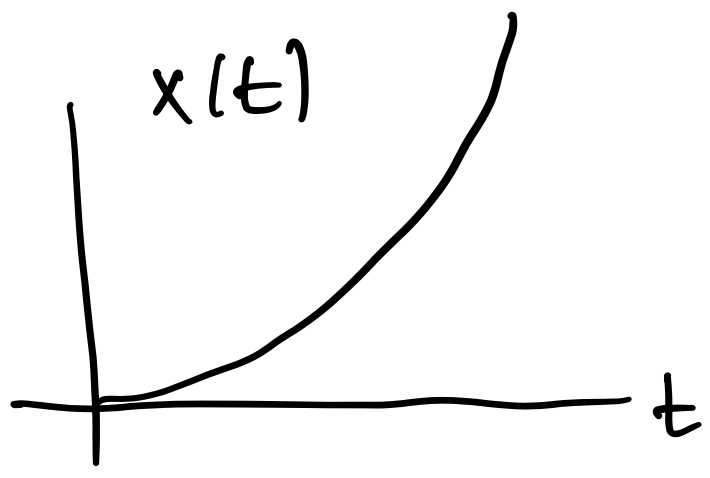
\includegraphics[width=0.8\linewidth]{../ExtFiles/PSet1-Q4b-a.png}
                    \caption{$|\gamma|>\omega_0$.}
                \end{subfigure}
                \begin{subfigure}[b]{0.3\linewidth}
                    \centering
                    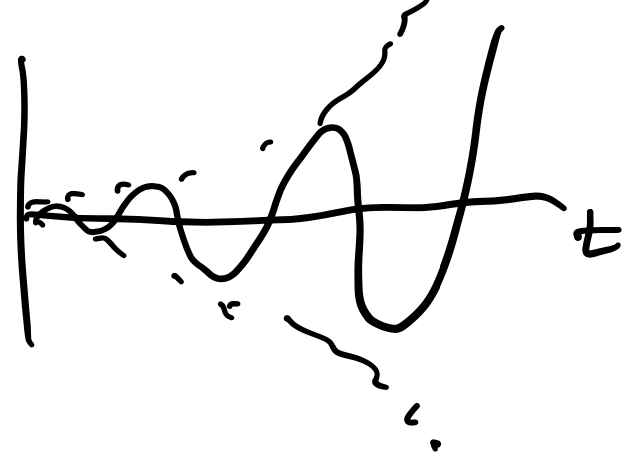
\includegraphics[width=0.8\linewidth]{../ExtFiles/PSet1-Q4b-b.png}
                    \caption{$|\gamma|<\omega_0$.}
                \end{subfigure}
                \begin{subfigure}[b]{0.3\linewidth}
                    \centering
                    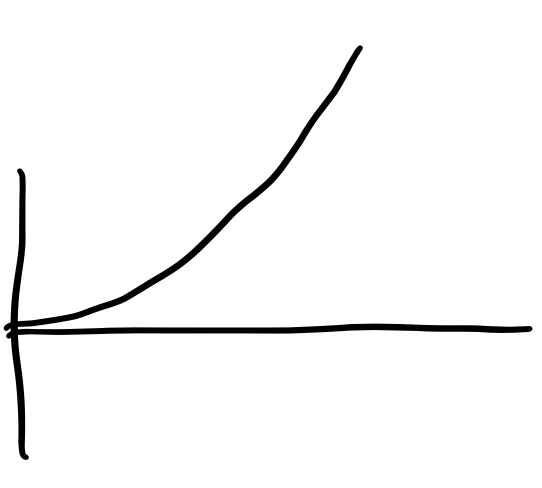
\includegraphics[width=0.8\linewidth]{../ExtFiles/PSet1-Q4b-c.png}
                    \caption{$\gamma=\omega_0$.}
                \end{subfigure}
            \end{figure}
            Case 1 ($|\gamma|>\omega_0$): In this case, the particle will diverge exponentially to $\infty$, briefly under the dominating $\gamma_-$ term and then under the dominating $\gamma_+$ term. Indeed, for $t\gg 1/\gamma_+$, we have
            \begin{equation*}
                x(t) \approx \frac{v}{\gamma_+-\gamma_-}\e[\gamma_+t]
            \end{equation*}
            Case 2 ($|\gamma|<\omega_0$): In this case, the particle will periodically oscillate while the oscillation's amplitude grows exponentially.\par
            Case 3 ($\gamma=\omega_0$): In this case, the particle will diverge exponentially to $\infty$, getting off to a quicker start because of its $t$ term but quickly losing the race to the larger $\gamma_+$ of Case 1.s
        \end{proof}
        \item In which case does the particle gain energy the fastest for large times? Explain. (2 pts)
        \begin{proof}
            We have that
            \begin{equation*}
                E = \frac{1}{2}m\dot{x}^2+\frac{1}{2}kx^2
            \end{equation*}
            Thus, the energy grows the fastest when $x,\dot{x}$ grow the fastest. In all three cases from part (b), both $x,\dot{x}$ grow exponentially (on average over a cycle). Eventually, these exponential rates will dominate over any differences in the prefactors. Notably, however, the \emph{largest} exponential rate is $\gamma_+=\gamma+\sqrt{\gamma^2-\omega^2}$ from the case where $|\gamma|>\omega_0$. Therefore, while a "positively damped" harmonic oscillator loses energy the fastest in the critically damped case, this "negatively damped" harmonically oscillating particle gains energy the fastest in this \fbox{overdamped case.}
        \end{proof}
    \end{enumerate}
    \item \textcite{bib:KibbleBerkshire}, Q2.25. For an oscillator under periodic force $F(t)=F_1\cos(\omega_1t)$\dots
    \begin{enumerate}
        \item Calculate the \textbf{power} (defined as the rate at which the force does work) of the periodic force. (4 pts)
        \begin{proof}
            From lecture, we know a particular solution of the driven, damped harmonic oscillator. It follows from the definition of power that we have
            \begin{align*}
                P &= F\dot{x}\\
                &= F_1\cos(\omega_1t)\dv{t}(a_1\cos(\omega_1t-\theta_1))\\
                \Aboxed{P &= -a_1\omega_1F_1\cos(\omega_1t)\sin(\omega_1t-\theta_1)}
            \end{align*}
        \end{proof}
        \item Show that the \textbf{average power} (defined as the time average over a complete cycle) of the periodic force is $m\omega_1^2a_1^2\gamma$, and hence verify that it is equal to the average rate at which energy is dissipated against the resistive force. (3 pts)
        \begin{proof}
            We approach this problem in two steps. Step 1 is to show that the average power of the periodic force is $\langle P_p\rangle=m\omega_1^2a_1^2\gamma$. Step 2 is to show that the average power of the resistive force is $\langle P_r\rangle=m\omega_1^2a_1^2\gamma$. Thus, we will have proven that these two powers are equal. Let's begin.\par\smallskip
            Step 1: Let $\tau$ be the period of the periodic force. Then its average power is given by
            \begin{equation*}
                \langle P_p\rangle = \frac{1}{\tau}\int_0^\tau P_p\dd{t}
            \end{equation*}
            Plugging in and solving, we can get to the following.
            \begingroup
            \allowdisplaybreaks
            \begin{align*}
                \langle P_p\rangle &= \frac{1}{\tau}\int_0^\tau F_1\cos(\omega_1t)\cdot -a_1\omega_1\sin(\omega_1t-\theta_1)\dd{t}\\
                &= -\frac{a_1\omega_1F_1}{\tau}\int_0^\tau\cos(\omega_1t)\sin(\omega_1t-\theta_1)\dd{t}\\
                &= -\frac{a_1\omega_1F_1}{\tau}\int_0^\tau\cos(\omega_1t)(\sin(\omega_1t)\cos\theta_1-\cos(\omega_1t)\sin\theta_1)\dd{t}\\
                &= -\frac{a_1\omega_1F_1}{\tau}\int_0^\tau\cos(\omega_1t)\sin(\omega_1t)\cos\theta_1\dd{t}+\frac{a_1\omega_1F_1}{\tau}\int_0^\tau\cos(\omega_1t)\cos(\omega_1t)\sin\theta_1\dd{t}\\
                &= -a_1\omega_1F_1\cos\theta_1\cdot\frac{1}{\tau}\int_0^\tau\cos(\omega_1t)\sin(\omega_1t)\dd{t}+a_1\omega_1F_1\sin\theta_1\cdot\frac{1}{\tau}\int_0^\tau\cos^2(\omega_1t)\dd{t}
            \end{align*}
            \endgroup
            At this point, we invoke the laws that
            \begin{align*}
                \int_0^\tau\cos(\omega_1t)\sin(\omega_1t)\dd{t} &= 0&
                \frac{1}{\tau}\int_0^\tau\cos^2(\omega_1t)\dd{t} &= \frac{1}{2}
            \end{align*}
            This simplifies the above expression to
            \begin{equation*}
                \langle P_p\rangle = \frac{a_1\omega_1F_1\sin\theta_1}{2}
            \end{equation*}
            But we're not quite done. Recalling that
            \begin{align*}
                \tan\theta_1 &= \frac{2\gamma\omega_1}{\omega_0^2-\omega_1^2}&
                \sin(\tan^{-1}(x)) &= \frac{x}{\sqrt{x^2+1}}
            \end{align*}
            we can learn that
            \begin{align*}
                \sin\theta_1 &= \frac{\frac{2\gamma\omega_1}{\omega_0^2-\omega_1^2}}{\sqrt{\left( \frac{2\gamma\omega_1}{\omega_0^2-\omega_1^2} \right)^2+1}}\\
                &= \frac{2\gamma\omega_1}{\sqrt{4\gamma^2\omega_1^2+(\omega_0^2-\omega_1^2)^2}}\\
                &= \frac{F_1/m}{\sqrt{(\omega_0^2-\omega_1^2)^2+4\gamma^2\omega_1^2}}\cdot\frac{2\gamma\omega_1}{F_1/m}\\
                &= \frac{2m\omega_1a_1\gamma}{F_1}
            \end{align*}
            Therefore, we have that
            \begin{align*}
                \langle P_p\rangle &= \frac{\omega_1a_1F_1}{2}\cdot\frac{2m\omega_1a_1\gamma}{F_1}\\
                &= m\omega_1^2a_1^2\gamma
            \end{align*}
            as desired.\par\smallskip
            Step 2: From the original driven, damped harmonic oscillator equation, we may read off that the resistive force is
            \begin{equation*}
                F_r = \lambda\dot{x}
            \end{equation*}
            Thus, its power is
            \begin{equation*}
                P_r = F_r\dot{x}
                = \lambda\dot{x}^2
                = 2m\gamma\cdot\omega_1^2a_1^2\sin^2(\omega_1t-\theta_1)
                = 2m\omega_1^2a_1^2\gamma\sin^2(\omega_1t-\theta_1)
            \end{equation*}
            Averaging once again, we obtain
            \begin{align*}
                \langle P_r\rangle &= \frac{1}{\tau}\int_0^\tau P_r\dd{t}\\
                &= 2m\omega_1^2a_1^2\gamma\cdot\frac{1}{\tau}\int_0^\tau\sin^2(\omega_1t-\theta_1)\dd{t}\\
                &= 2m\omega_1^2a_1^2\gamma\cdot\frac{1}{2}\\
                &= m\omega_1^2a_1^2\gamma
            \end{align*}
            as desired.
        \end{proof}
        \item Show that the average power from part (b) --- as a function of $\omega_1$ --- is at a maximum at $\omega_1=\omega_0$. Also find the values of $\omega_1$ for which it has half its maximum value. (3 pts)
        \begin{proof}
            To prove that $\langle P\rangle(\omega_1)$ has a maximum at $\omega_1=\omega_0$, it will suffice to show that
            \begin{align*}
                \eval{\dv{\langle P\rangle}{\omega_1}}_{\omega_1=\omega_0} &= 0&
                \eval{\dv[2]{\langle P\rangle}{\omega_1}}_{\omega_1=\omega_0} &< 0
            \end{align*}
            We will prove the equality on the left first. Let's begin. From part (b) and the definition of $a_1$ from class, we have that
            \begin{equation*}
                \langle P\rangle = m\omega_1^2a_1^2\gamma
                \propto \frac{\omega_1^2}{(\omega_0^2-\omega_1^2)^2+4\gamma^2\omega_1^2}
            \end{equation*}
            Thus, since constants factor out of derivatives, checking the left expression below will suffice to confirm the right expression below.
            \begin{equation*}
                \eval{\dv{\omega_1}\left[ \frac{\omega_1^2}{(\omega_0^2-\omega_1^2)^2+4\gamma^2\omega_1^2} \right]}_{\omega_1=\omega_0} = 0
                \qquad\Longrightarrow\qquad
                \eval{\dv{\langle P\rangle}{\omega_1}}_{\omega_1=\omega_0} = 0
            \end{equation*}
            We now introduce the substitutions
            \begin{align*}
                u &= \omega_1^2&
                v &= \omega_0^2&
                C &= 4\gamma^2
            \end{align*}
            Thus,
            \begin{equation*}
                \langle P\rangle \propto \frac{u}{(v-u)^2+Cu}
            \end{equation*}
            Moreover, since the chain rule implies that
            \begin{equation*}
                \dv{\omega_1}\left[ \frac{\omega_1^2}{(\omega_0^2-\omega_1^2)^2+4\gamma^2\omega_1^2} \right] = \dv{u}\left[ \frac{u}{(v-u)^2+Cu} \right]\cdot\dv{u}{\omega_1}
            \end{equation*}
            we need only check that
            \begin{equation*}
                \eval{\dv{u}\left[ \frac{u}{(v-u)^2+Cu} \right]}_{u=v} = 0
            \end{equation*}
            We can do this as follows.
            \begin{align*}
                \eval{\dv{u}\left[ \frac{u}{(v-u)^2+Cu} \right]}_{u=v} &= \eval{\frac{[(v-u)^2+Cu]\cdot[1]-[u]\cdot[-2(v-u)+C]}{[(v-u)^2+Cu]^2}}_{u=v}\\
                &= \frac{[(v-v)^2+Cv]\cdot[1]-[v]\cdot[-2(v-v)+C]}{[(v-v)^2+Cv]^2}\\
                &= \frac{0}{(Cv)^2}\\
                &= 0
            \end{align*}
            For analogous reasons to above, to check the right equality at the top, it will suffice to show that
            \begin{equation*}
                \eval{\dv[2]{u}\left[ \frac{u}{(v-u)^2+Cu} \right]}_{u=v} < 0
            \end{equation*}
            We can do this as follows.
            \begingroup
            \allowdisplaybreaks
            \begin{align*}
                \eval{\dv[2]{u}\left[ \frac{u}{(v-u)^2+Cu} \right]}_{u=v}\hspace{-7em}\\
                &= \eval{\dv{u}\left\{ \frac{v^2-u^2}{[(v-u)^2+Cu]^2} \right\}}_{u=v}\\
                &= \eval{\frac{[(v-u)^2+Cu]^2\cdot[-2u]-[v^2-u^2]\cdot[2((v-u)^2+Cu)(-2(v-u)+C)]}{[(v-u)^2+Cu]^2}}_{u=v}\\
                &= \frac{[(v-v)^2+Cv]^2\cdot[-2v]-[v^2-v^2]\cdot[2((v-v)^2+Cv)(-2(v-v)+C)]}{[(v-v)^2+Cv]^2}\\
                &= -2v\\
                &< 0
            \end{align*}
            \endgroup
            Now for the final part of the problem. As before, we can keep working with our proportional function in $u,v,C$. This function can be rewritten as follows.
            \begin{equation*}
                \frac{u}{(v-u)^2+Cu} = \frac{1}{\frac{1}{u}(v-u)^2+C}
            \end{equation*}
            The expression on the right above is clearly maximized when $(v-u)^2/u=0$.\footnote{Note that this would have been a way to prove that maximization without using calculus.} Similarly, the half-maximum occurs when $(v-u)^2/u=C$. But this only occurs when
            \begin{align*}
                uC &= v^2-2uv+u^2\\
                0 &= u^2+(-2v-C)u+v^2\\
                u &= \frac{-(-2v-C)\pm\sqrt{(-2v-C)^2-4v^2}}{2}\\
                &= \frac{2v+C\pm\sqrt{4vC+C^2}}{2}\\
                \omega_1^2 &= \frac{2\omega_0^2+4\gamma^2\pm\sqrt{16\omega_0^2\gamma^2+16\gamma^4}}{2}\\
                &= \omega_0^2+2\gamma^2\pm 2\gamma\sqrt{\omega_0^2+\gamma^2}\\
                &= \left( \gamma\pm\sqrt{\omega_0^2+\gamma^2} \right)^2\\
                \Aboxed{\omega_1 &= \gamma\pm\sqrt{\omega_0^2+\gamma^2}}
            \end{align*}
            Note that we neglect the negative solutions --- that is, $-(\gamma\pm\sqrt{\omega_0^2+\gamma^2})$ --- because in physical reality, $\omega_1\not<0$.
        \end{proof}
    \end{enumerate}
    \item \textcite{bib:KibbleBerkshire}, Q2.32. Find the Green's function of an oscillator in the case $\gamma>\omega_0$. Use it to solve the problem of an oscillator that is initially in equilibrium, and is subjected from $t=0$ to a force increasing linearly with time via $F=ct$.
    \item How long did you spend on this problem set?
    \begin{proof}
        About 10 hours.
    \end{proof}
\end{enumerate}




\end{document}